\section{Non-inverting Amplifier}


%%%%%%%%%%%%%%%%%%%%%%%%%%%%%%%%%%%%%%%%%%%%%%%%%%%%%
\subsection{Pengantar Non-Inverting Amplifier}

\begin{frame}{Pengantar Non-inverting Amplifier}
	\begin{itemize}
		\item Non-inverting amplifier adalah salah satu rangkaian op amp dasar.
		\item Non-inverting amplifier menggunakan negative feedback untuk menstabilkan overall voltage gain.
		\item Dengan amplifier jenis ini, negative feedback juga meningkatkan impedansi input dan menurunkan impedansi output.
	\end{itemize}
\end{frame}


%%%%%%%%%%%%%%%%%%%%%%%%%%%%%%%%%%%%%%%%%%%%%%%%%%%%%

\subsection{Rangkaian Dasar}
\begin{frame}{Rangkaian Dasar}
	\begin{figure}
		\centering
		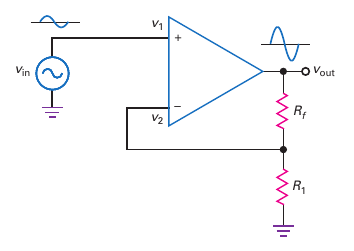
\includegraphics[width=0.5\linewidth]{gambar/fig-16.18}
		\caption{Non-inverting amplifier}
		\label{fig-16.18}
	\end{figure}
\end{frame}

\begin{frame}{Rangkaian Dasar}
	\begin{itemize}
		\item Gambar \ref{fig-16.18} menunjukkan rangkaian ekivalen ac dari noninverting amplifier.
		\item Tegangan input ($ v_{in} $) men-drive noninverting input.
		\item Tegangan input ini dikuatkan untuk menghasilkan tegangan output se-fasa (Seperti yang ditunjukkan oleh Gambar \ref{fig-16.18}).
		\item Tegangan output diumpanbalikan ke input melalui pembagi tegangan.
		\item Tegangan sepanjang $ R_1 $ adalah tegangan feedback yang diberikan ke inverting input.
		\item Tegangan feedback ini hampir sama dengan tegangan input.
		\item Karena open-loop voltage gain yang besar, perbedaan antara $ v_1 $ dan $ v_2 $ sangat kecil.
		\item Karena tegangan feedback berlawanan dengan tegangan input, maka kita mendapatkan negative-feedback.
	\end{itemize}
\end{frame}

\begin{frame}{Rangkaian Dasar}
	\begin{itemize}
		\item Bagaimana negative-feedback dapat menstabilkan keseluruhan voltage gain?
		\item Jika open-loop voltage gain ($ A_{VOL} $) meningkat, tegangan output akan meningkat dan lebih banyak tegangan feedback ke inverting input.
		\item Tegangan feedback yang berkebalikan ini yang akan mereduksi tegangan input ($ v_1 - v_2 $).
		\item Sehingga, meskipun $ A_{VOL} $ meningkat, $ v_1 - v_2 $ akan berkurang, dan output akhir meningkat jauh lebih sedikit daripada jika tidak ada negative feedback. 
		\item Overall output (tegangan output) hanya sedikit peningkatan.
	\end{itemize}
\end{frame}


%%%%%%%%%%%%%%%%%%%%%%%%%%%%%%%%%%%%%%%%%%%%%%%%%%%%%

\subsection{Virtual Short}

\begin{frame}{Virtual Short}
	\begin{itemize}
		\item Saat kita menghubungkan dua titik dalam rangkaian dengan kabel, tegangan kedua titik tersebut terhadap ground akan bernilai sama.
		\item Kabel tersebut memberikan jalur kepada arus untuk mengalir antara dua titik tersebut.
		\item Mechanical short (kabel yang menghubungkan 2 titik) adalah hubungan singkat (short) untuk tegangan maupun arus.
	\end{itemize}
\end{frame}

\begin{frame}{Virtual Short}
	\begin{itemize}
		\item Virtual short digunakan untuk menganalisis noninverting amplifier dengan cepat dan mudah.
		\item Virtual short menggunakan 2 sifat dari op amp ideal:
		
		\begin{enumerate}
			\item Ketika $ R_{in} $ adalah tak hingga, kedua arus input adalah nol.
			\item Ketika $ A_{VOL} $ adalah tak hingga, $ v_1 - v_2 $ adalah nol.
		\end{enumerate}
		
		\item Gambar \ref{fig-16.19} menunjukkan virtual short antara terminal input op amp.
		
	\end{itemize}
\end{frame}

\begin{frame}{Virtual Short}
	\begin{figure}
		\centering
		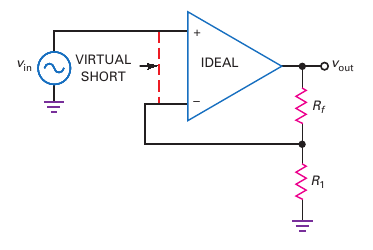
\includegraphics[height=0.7\textheight]{gambar/fig-16.19}
		\caption{Virtual short}
		\label{fig-16.19}
	\end{figure}
\end{frame}

\begin{frame}{Virtual Short}
	\begin{itemize}
		\item Virtual short adalah short untuk tegangan tetapi open untuk arus.
		\item Garis putus-putus menandakan tidak ada arus yang mengalir.
		\item Meskipun virtual short merupakan pendekatan yang ideal, metode ini memberikan jawaban yang lebih akurat ketika digunakan dengan heavy negative feedback.
	\end{itemize}
\end{frame}

\begin{frame}{Virtual Short}
	\begin{itemize}
		\item Bagaimana cara menggunakan virtual short?
		\item Kapan pun kita menganalisa inverting amplifier atau rangkaian yang semisal, kita dapat memvisualisasikan virtual short antara terminal input dari op amp.
		\item Selama op amp beroperasi secara linear (tidak saturasi positif maupun negatif), open-loop voltage gain mendekati tak hingga dan virtual short berada di antara kedua input terminal.
		\item Hal yang perlu diperhatikan: karena virtual short, tegangan input inverting mengikuti tegangan input noninverting. Jika tegangan noninverting input meningkat atau menurun, seketika tegangan input inverting akan meningkat atau menurun. Peristiwa ini disebut dengan \textbf{bootstrapping}
	\end{itemize}
\end{frame}


%%%%%%%%%%%%%%%%%%%%%%%%%%%%%%%%%%%%%%%%%%%%%%%%%%%%%

\subsection{Voltage Gain}

\begin{frame}{Voltage Gain}
	\begin{itemize}
		\item Gambar \ref{fig-16.20} menunjukkan virtual short antara terminal input op amp.
		\item Artinya tegangan input ada di $ R_1 $, sehingga dapat kita tuliskan:\\
		
		\[ v_{in} = i_1 R_1 \]
		
		\item Karena tidak ada arus yang mengalir melalui virtual short, arus $ i_1 $ juga mengalir di $ R_f $, yang artinya teganan output yang dihasilkan:\\
		
		\[ v_{out} = i_1 (R_f + R_1) \]
		
		\item Untuk mendapatkan voltage gain maka $ v_{out} $ dibagi oleh $ v_{in} $:\\
		
		\begin{equation}\label{pers.16.12}
			A_{v(CL)} = \frac{R_f + R_1}{R_1} = \frac{R_f}{R_1} + 1
		\end{equation}
	
	\end{itemize}
\end{frame}

\begin{frame}{Voltage Gain}
	\begin{figure}
		\centering
		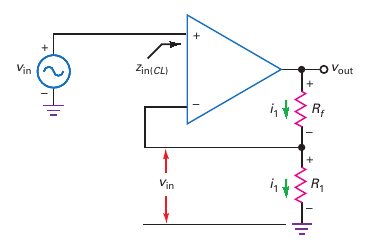
\includegraphics[width=\linewidth]{gambar/fig-16.20}
		\caption{Tegangan input ada di $ R_1 $ dan arus yang sama mengalir di $ R_1 $}
		\label{fig-16.20}
	\end{figure}
\end{frame}

\subsection{Impedansi Input, Bandwidth, Bias \& Offset}
\begin{frame}{Impedansi Input, Bandwidth, Bias \& Offset}
	\begin{itemize}
		\item Karena impedansi input open-loop sudah sangat besar (2 M$ \Omega $ untuk 741C), maka impedansi input closed-loop lebih besar lagi.
		\item Efek negative feedback terhadap bandwidth sama seperti di inverting amplifier
		\[ f_{2(CL)} = \frac{f_{unity}}{A_{v(CL)}} \]
		\item Efek bias dan offset juga sama seperti di inverting amplifier
	\end{itemize}
\end{frame}

\subsection{Error Tegangan Output Mereduksi MPP}
\begin{frame}{Error Tegangan Output Mereduksi MPP}
	\begin{figure}
		\centering
		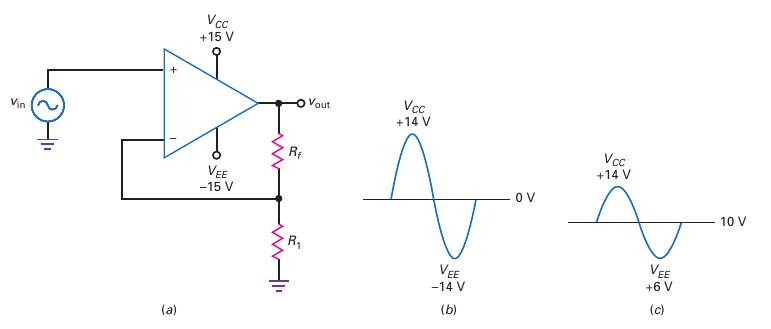
\includegraphics[width=0.9\linewidth]{gambar/fig-16.21}
		\caption{Error tegangan output dapat mereduksi MPP}
		\label{fig-16.21}
	\end{figure}
\end{frame}

\subsection{Contoh Soal 2.10}
\begin{frame}{Contoh Soal 2.10}
	\begin{multicols}{2}
		\begin{center}
			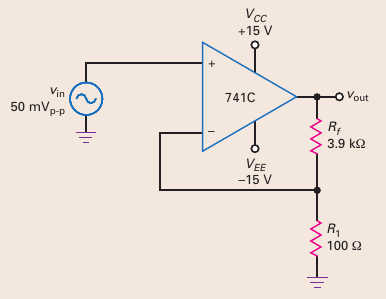
\includegraphics[width=\linewidth]{gambar/fig-16.22a}
		\end{center}
		\columnbreak
		\begin{itemize}
			\item Pertanyaan:
			\begin{itemize}
				\item Berapa penguatan tegangan closed-loop dan bandwidth?
				\item Berapa tegangan output di 250 kHz?
			\end{itemize}
		\end{itemize}
	\end{multicols}
\end{frame}

\begin{frame}{Contoh Soal 2.10}
	\begin{multicols}{2}
		\begin{center}
			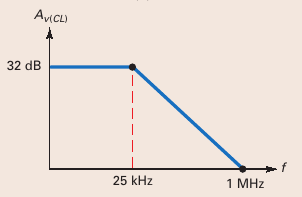
\includegraphics[width=0.8\linewidth]{gambar/fig-16.22b}
		\end{center}
		\columnbreak
		\begin{itemize}
			\item Jawaban:
			\begin{itemize}
				\item Penguatan tegangan closed-loop:
				\begin{align*}
					A_{v(CL)} &= \frac{R_f}{R_1} + 1 = \frac{3.9 \text{ k}\Omega}{100 \text{ k}\Omega} + 1 = 40
				\end{align*}
				\item Bandwidth:
				\begin{align*}
					f_{2(CL)} = \frac{f_{unity}}{A_{v(CL)}} = \frac{1 \text{ MHz}}{40} = 25 \text{ kHz}
				\end{align*}
				\item Tegangan output di 250 kHz
				\begin{align*}
					v_{out} &= A_{c(CL)} v_{in} = 4(50 \text{ mVp-p})\\
					&= 200 \text{ mVp-p}
				\end{align*}
			\end{itemize}
		\end{itemize}
	\end{multicols}
\end{frame}

\subsection{Latihan Soal 2.10}
\begin{frame}{Latihan Soal 2.10}
	\begin{multicols}{2}
		\begin{center}
			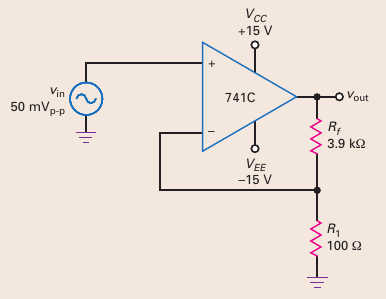
\includegraphics[width=\linewidth]{gambar/fig-16.22a}
		\end{center}
		\columnbreak
		\begin{itemize}
			\item Pertanyaan:
			\begin{itemize}
				\item Jika $ R_f = 4.9 \text{ k}\Omega $, tentukan $ A_{v(CL)} $ dan $ v_{out} $ di 200 kHz.
			\end{itemize}
		\end{itemize}
	\end{multicols}
\end{frame}

\subsection{Contoh Soal 2.11}
\begin{frame}{Contoh Soal 2.11}
	\begin{multicols}{2}
		\begin{center}
			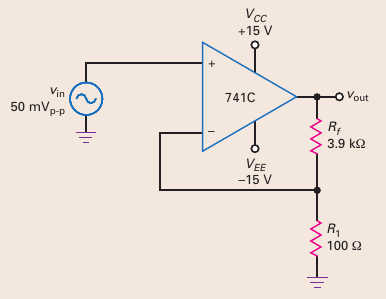
\includegraphics[width=\linewidth]{gambar/fig-16.22a}
		\end{center}
		\columnbreak
		\begin{itemize}
			\item Pertanyaan:
			\begin{itemize}
				\item Jika $ I_{in(bias)} = 500 \text{ nA} $, $ I_{in(off)} = 200 \text{ nA} $, dan $ V_{in(off)} = 6 \text{ mV} $, berapa error tegangan output?
			\end{itemize}
		\end{itemize}
	\end{multicols}
\end{frame}

\begin{frame}{Contoh Soal 2.11}
	\begin{multicols}{2}
		\begin{center}
			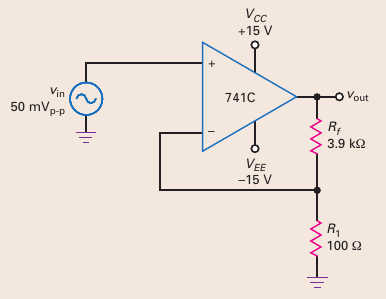
\includegraphics[width=\linewidth]{gambar/fig-16.22a}
		\end{center}
		\columnbreak
		\begin{itemize}
			\item Jawaban:
			\begin{itemize}
				\item Resistor Thevenin:
				\begin{align*}
					R_{B2} &= R_1 \parallel R_f = 3.9 \text{ k}\Omega \parallel 100~\Omega \\
					R_{B2} &\approx 100~\Omega
				\end{align*}
				\item Error tegangan input
				\begin{align*}
					V_{1err} &= (R_{B1} - R_{B2})I_{in(bias)}  \\
					&= (-100~\Omega)(500 \text{ nA}) = -0.05 \text{ mV}\\
					V_{2err} &= (R_{B1} + R_{B2})I_{in(bias)} \\
					&= (100~\Omega)(100 \text{ nA}) = 0.01 \text{ mV}\\
					V_{3err} &= V_{in(off)} = 6 \text{ mV}
				\end{align*}
			\end{itemize}
		\end{itemize}
	\end{multicols}
\end{frame}

\begin{frame}{Contoh Soal 2.11}
	\begin{multicols}{2}
		\begin{center}
			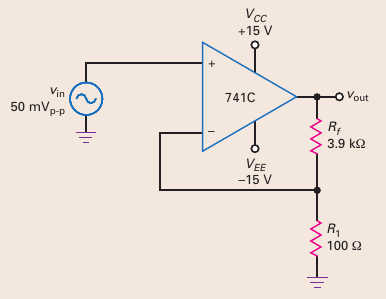
\includegraphics[width=\linewidth]{gambar/fig-16.22a}
		\end{center}
		\columnbreak
		\begin{itemize}
			\item Jawaban:
			\begin{itemize}
				\item Error tegangan output
				\begin{align*}
					V_{error} &= \pm A_{v(CL)}(\pm V_{1err} \pm V_{2err} \pm V_{3err}) \\
					&= \pm 40 (0.05 \text{ mV} + 0.01 \text{ mV} + 6 \text{ mV}) \\
					&= \pm 242 \text{ mV}
				\end{align*}
			\end{itemize}
		\end{itemize}
	\end{multicols}
\end{frame}